\documentclass{article}
\usepackage{graphicx}
\usepackage{wrapfig}
\usepackage{caption}
\usepackage{subcaption}
\usepackage[spanish, es-tabla]{babel}
\renewcommand{\baselinestretch}{1.5}
\usepackage[backend=bibtex,sorting=none]{biblatex}
\bibliography{bibliography}
\usepackage[noend]{algpseudocode}
\usepackage{algorithm}


\algnewcommand\algorithmicforeach{\textbf{for each}}
\algdef{S}[FOR]{ForEach}[1]{\algorithmicforeach\ #1\ \algorithmicdo}
\algnewcommand\algorithmicyield{\textbf{yield}}
\algnewcommand\yield{\item[\algorithmicyield]}

\begin{document}
		
	\begin{titlepage}
		\centering
		{
\includegraphics[width=0.2\textwidth]{logo}\par}
		\vspace{1cm}
		{\bfseries\LARGE Instituo Tecnológico de Oaxaca \par}
		\vspace{1cm}
		{\scshape\Large Ingeniería en Sistemas Computacionales  \par}
		\vspace{1cm}
		{\scshape\Huge Simulación de difusión activa y pasiva en redes
			complejas \par}
		\vspace{3cm}
		\vfill
		{\Large Autor: \par}
		{\Large José Ángel García García \par}
		\vfill
		{\Large Enero 2021 \par}
		\end{titlepage}
	
\tableofcontents
\newpage
	
\section{Selección de Modelo}	
Antes de explicar a detalle el trabajo realizado, se debe recalcar que para elegir este modelo se realizaron diferentes actividades. Y se enlista a continuación las hojas que contiene el documento de calculo en el que se puede encontrar el filtrado realizado \cite{filtros:2020}.
\begin{itemize}
	\item \textbf{Busqueda}: Se plasman los 100 modelos de simulación buscados.
	\item \textbf{Filtro-1}: Se eligen los modelos de simulación que más me hayan llamado la atención.
	\item \textbf{Filtro-2}: Se evalua los modelos del filtro anterior para ver la viabilidad de conseguir los datos.
	\item \textbf{Filtro-3}: Se examinan las variables de los modelos que pasaron hasta este filtro, para analizar la dificultad de su implementación.
	\item \textbf{Filtro-3.2}: Se realiza el mismo filtro, examinando a mayor detalle.
	\item \textbf{Filtro-3.3}: Se vuelve a aplicar el mismo filtro pero ahora intento explicar el modelo para ver si se entiende con claridad y optar por los más precisos.
	\item \textbf{Filtro-4}: Se clasifican los modelos, debido a que algunos son de la misma área, en este punto tenía modelos de colas y de grafos.
	\item \textbf{Elegido}: Se plasma el modelo elegido, que es el descrito a continuación.
\end{itemize}

\section{Introducción}
 La información, las ideas, los virus, todos ellos tienen algo en común: describen diferentes tipos de “contenidos” que necesitan ser vinculaos por agentes interactuantes para difundirse. Estos agentes pueden ser animales, personas o cualquier otro ser vivo, inclusive una computadora o dispositivos tecnológicos conectados por una red compleja que describe sus relaciones. Los procesos de difusión presentan características que afectan la forma en que evolucionan, una de esas características es el \textbf{grado de actividad} de sus agentes, donde esto puede ser \textbf{pasivo} y \textbf{activo}, aunque en algunos casos pueden tomar ambos comportamientos. Además, en determinadas circunstancias, un contenido puede necesitar tanto de un cierto grado de exposición de los actores como su interés para ser tomado en cuenta.
 \\
 La distinción de actividad se refiere a fenómenos de contagio social, donde el objeto de difusión o difuso es una idea o un dato. Los contagios sociales se suelen modelar utilizando un enfoque clásico con el modelo \textbf{Threshold} introducido por Granovetter en 1978 \cite{granovetter:1978}.
 Este modelo, la adopción de ideas o información por un individuo está sujeta a un umbral personal, además que tienden a considerar solo el componente pasivo de la difusión, ignorando los intereses del usuario en relación con la información.
 Sabemos que la presión en grupo en la mayoría de agentes puede ser un factor para la adopción de información, pero hay casos en los que el interés personal es más relevante, un impulso activo, que una vez el agente es consciente de la existencia de la información, sin tener en cuenta la presión de su exterior u otros agentes puede aceptar o declinar el proceso de difusión.
 \\
 Actualmente, no existen modelos que consideren a los usuarios activos y pasivos en al difusión de una red. Y en el mundo real, los usuarios tienen este comportamiento, por ejemplo, algunas personas que deciden de forma autónoma adoptar una idea o información sin la presión de sus amigos y otras que deciden no adoptar esas ideas. Entonces, en este trabajo, modelamos también el fenómeno de adopción espontánea y la presencia de nodos bloqueados. Una distinción simple que se realiza en el presente documento, es que el modelado \textbf{pasivo} se trabaja mediante reglas de difusión deterministas(umbrales individuales que limitan los fenómenos de presión de grupo) y \textbf{activo} a través de probabilísticos (perfiles individuales que dependen únicamente del interés del sujeto en el contenido o información).
 \subsection{Planteamiento del problema}
Los procesos de difusión se pueden dividir en tres componentes: (i) la población sobre la que se desenvuelven, (ii) los mecanismos que describen su evolución y (iii) el contenido de la difusión. Todos esos  componentes son igualmente importantes para modelar, comprender, simular un proceso de difusión: en particular, la difusión del contenido representa el discriminante real entre difusión activa / pasiva. 
Se suele decir "Propagación de la epidemia" para referirse a difusiones de enfermedades contagiososas originadas por patógenos biológicos. Sin embargo, una plétora de fenómenos pueden vincularse al concepto de epidemia: ejemplos son la propagación de virus informáticos \cite[Szor 2004]{Szor:2004}, así como la  propagación del virus del teléfono móvil \cite[Havlin 2009]{Haviln:2009}, \cite[Wang 2013]{Wang:2013}, o la difusión de conocimientos, innovaciones, productos en una red social online \cite[Burt 1987]{Burt:1987}.

Destacando de estas, su representación mediante redes complejas donde los nodos se caracterizan por su estado infeccioso e interpretan a los agentes, y los enlaces representan la interacción entre nodos.
\\
En el presente articulo se considera especificamente la difusión: innovaciones/ideas. La difusión de la teoría de la innovación, desarrollada por Rogers en 1962 \cite*{rogers:2003} es una de las teorias de las ciencias sociales más antiguas: tiene como objetivo explicar cómo una idea o producto gana fuerza y se difunde a través de una publicación o red. La adopción de una nueva idea, comportamiento, producto, información,etc. no ocurre de forma simultanea en un sistema social, es todo un proceso en el que algunas personas son más adecuadas para adoptar la innovación que otras. El problema de la difusión de la innovación se aborda mediante variantes del \textbf{Modelo Treshold}, en dicho modelo se tiene dos alternativas l comportamientos distintas y mutuamente excluyentes, la decisión de hacer o no hacer algo, una decisión vinculada a cuantas otras personas han tomado la misma decisión, es decir, está influenciada por el un grupo de personas y esto es conocido como presión social. En \cite[Watts 2002]{watts:2002}, se demostró que al aplicar dicho modelo en una red, puede ocurrir una cascada de difusión global debido a las interacciones entre los nodos y los threshold individuales. Sin embargo, tal modelo presenta algunas limitaciones: 

\begin{itemize}
	\item No considera los impulsos externos que pueden llegar desde los medios de comunicación, publicidad, amigos, etc.
	\item No considera a la presencia de individuos reacios (resistentes) a adoptar.
\end{itemize}

Recientemente también se investigó el efecto de la hemofilia \cite[Aral 2009]{aral:2009}, \Cite[Bakshy 2012]{bakshy:2012}, \cite[Watts 2011]{watts:2011} y el papel de la influencia de los medios externos \cite[Toole 2012]{toole:2012}. Por el contrario, la presencia de personas reacias se abordó en \cite[Ruan 2015]{ruan:2015} donde se introdujo un modelo basado en threshold que incluye nodos bloqueados así como adoptantes espontáneos.
\\
En este trabajo se introdujeron dos enfoques cuyo objetivo es proporcionar esquemas activos y mixtos aplicables en el contexto de la simulación de innovaciones/conductas/difusión de ideas en el caso estático, introduciendo también el concepto de nodos bloqueados.

En este trabajo, se usa una tipología particular de difusión en red, la difusión de innovaciones$/$comportamientos$/$ideas, la difusión de innovaciones se utiliza para describir un proceso activo, cada agente decide de forma autónoma adoptar$/$publicitar un contenido determinado. La difusión de información y la propagación de una epidemia se distinguen fácilmente por el grado de actividad de los individuos que afectan.\\ 
Tal dicotomía dependiente del contexto conduce a nuestra definición de problema:\\

\textbf{Definicion 1}(Enigma activo-pasivo) Dado un \textbf{contexto social} descrito como un gráfico $G = (V, E)$, donde un nodo $v \in V$ es un individuo y ua arista $(u, v) \in E$ identifica un lazo social entre $u$, $v \in V - a$ \textbf{contenido $\psi$} y un conjunto de adoptantes que $t_0 \subset V$: ¿Cómo pueden modelarse y qué caracterizan los procesos de difusión pasiva y activa de $\psi$ sobre $G$?.
 
\section{Diseño del Modelo}
Para abordar fenómenos difusivos relacionados con la tipología de contenidos que nos interesan en este trabajo se suelen adoptar variantes del \textbf{Modelo Threshold} en el que las adopciones realizadas por los individuos están sujetos a threshold personales (identificada como la presión social). Estos enfoques se centran en capturar el componente \textbf{pasivo} de la difusión, ignorando el interés del usuario por el contenido $\psi$.
\subsection{Formulación del modelo}
Dado que nuestro objetivo es comparar opciones de modelado alternativas capaces de simular tanto pasivo y/o activo Los procesos de difusión primero necesitamos caracterizar los escenarios que tales enfoques deberían describir.
\begin{itemize}
	\item \textbf{S1: Difusión pasiva.} Este escenario asume que un proceso de difusión genérico se lleva a cabo independientemente de la voluntad de los individuos. La difusión se basa solo en la presión de grupo, el contagio socialactúaa como lapropagaciónn del virus, ya que, alcanzada una presión suficiente de compañeros, la difusión del contenido afectará al usuario sin considerar sus preferencias individuales.
	\item \textbf{S2: Difusión activa.} 
	Continuar escribiendo
	A la inversa del escenario de difusión pasiva, la difusión activa supone que el proceso de difusión es solo aparente; cada individuo decide adoptar o no un contenido determinado, se basa únicamente en el interés del individuo, descartando por completo la presión social.
	\item \textbf{S3: Difusión mixta.} Este escenario combina procesos pasivo y activo para dar la forma a la difusión de información como una mezcla de ambos.
\end{itemize}
A continuación, detallaremos las elecciones algorítmicas realizadas para proporcionar simulaciones de los escenarios esbozados considerando la presencia/ausencia de adopciones espontáneas y la presencia/ausencia de nodos bloqueados.	

\subsection{Explicación del modelo}
Para entender las diferencias entre los escenarios propuestos se simularon con los siguientes modelos de difusión:
\begin{itemize}
 \item \textbf{S1: Threshold model.} Empleamos el clásico Modelo de Thresgold (Granovetter 1978) para simular un \textbf{adopción pasiva} proceso mediante el uso de una distribución teórica para el threshold de adopción como se hace en \cite[Watts 2002]{watts:2002}. Un nodo tiene dos alternativas de comportamiento distintas y mutuamente excluyentes, por ejemplo, puede adoptar o no el contenido difundido, la decisión de adoptar depende solo del porcentaje de vecinos del nodo que ya han adoptado el contenido.
 
  
 \begin{algorithm} 
 	\caption{Algorithm 1: Threshold}
 	\begin{algorithmic}[1]	
 		\Require {$I_{t_0}$: seeds de infectados, $k$: número de iteraciones, $\tau$: umbrales del nodo}
 	\ForEach {$t_i \in \{1,...,k\} $}
 		\State {$I_{t_i}=I_{t_{i-1}}$}
 		\ForEach {$n \in V $}
 			\If {$n \not \in I_{t_{i-1}}$ $and$ $neighbors(n)\cap I_{t_{i-1}} \neq \emptyset$}
 			\State {$\lambda_n = |neighbors(n)\cap I_{t_{i-1}}|$}
 			\If{$\lambda_n \geq \tau_n$}
 			\State {add $n$ to $I_{t_i}$}
 			\EndIf
 			\EndIf
	\\ \textbf{$.....$yield} $I_{t_i}$
	 \EndFor
	 \EndFor			
 	\end{algorithmic}
 \end{algorithm}
 
 \item \textbf{S2: Node Profile model.}
Para simular el activo de adopciones, cada adoptante elige adoptar el contenido dado basándose únicamente en sus preferencias personales. Cada nodo lleva su perfil $\iota$ describiendo el grado en que es probable que acepte un contenido similar al que se está difundiendo actualmente. El proceso de difusión parte de un conjunto de nodos que ya han adoptado el contenido $\psi$. Para cada uno de los nodos susceptibles en la vecindad de un nodo $n$ que ya ha adoptado $\psi$, un valor aleatorio $v$ en $[0,1]$ se extrae; Si $v \geq \iota_n$ el nodo adopta el contenido, de lo contrario, el nodo se niega a adoptar. Los nodos susceptibles pueden cambiar de opinión durante cada iteración. También implementamos una variante de dicho modelo que contempla nodos bloqueados, por ejemplo, nodos que luego de haber rechazado la adopción, con probabilidad $p$ deciden seguir con sus elecciones de forma permanente. 

\begin{algorithm} 
	\caption{Node Profile}
	\begin{algorithmic}[1]	
		\Require {$I_{t_0}$: seeds de infectados; $k$: número de iteraciones, $\gamma$: perfiles del nodo, $p$: probabilidad de inmunización}
		\State {$B = \{\}$}
		\ForEach {$t_i \in \{1,...,k\} $}
		\State {$I_{t_i}=I_{t_{i-1}}$}
		\ForEach {$n \in V $}
		\If {$n \not \in I_{t_{i-1}}$ $and$ $n \not \in B$ $and$ $neighbors(n)\cap I_{t_{i-1}} \neq \emptyset$}
		\State $r_n = rand(0,1)$
		\If{$r_n \geq \gamma_n$}
		\State {add $n$ to $I_{t_i}$}
		\Else 
			\State $ q = rand(0,1)$
			\If{$q \leq p$}
			\State add $n$ to $B$
			\EndIf
		\EndIf
		\EndIf
		\EndFor
	\\ \textbf{$.....$yield} $I_{t_i}, B$
	
	\EndFor
	\end{algorithmic}
\end{algorithm}

 \item \textbf{S3: Profile-Threshold model.}
Para modelar los comportamientos mixtos, implementamos un $Node$ $Profile$$-$$Threshold$, un modelo que combina el $Node$ $Profile$ $model$ descrito anteriormente con la información de presión de grupo (es decir, $Threshold$ $model$ clásico). En primer lugar, este modelo evalúa si la presión de grupo que recibe un nodo es suficiente para superar su $Threshold$, luego, si se satisface dicha restricción, evalúa el perfil del nodo. En cuanto al modelo $Node$ $Profile$, implementamos una variante que contempla los nodos bloqueados. 

Para modelar las adopciones espontáneas, se introdujo, como primer paso antes de cada iteración de simulación, un proceso estocástico nodal que con una probabilidad fija $p$ transforma un nodo susceptible en uno infectado.
\begin{algorithm} 
	\caption{Profile - Threshold}
	\begin{algorithmic}[1]	
		\Require {$I_{t_0}$: seeds de infectados; $k$: número de iteraciones, $\tau$: umbrales del nodo, $\gamma$: perfiles del nodo, $p$: probabilidad de inmunización}
		\State {$B$ = $\{$$\}$}
		\ForEach {$t_i \in \{1,...,k\} $}
		\State {$I_{t_i}=I_{t_{i-1}}$}
		\ForEach {$n \in V $}
		\If {$n \not \in I_{t_{i-1}}$ $and$ $n \not \in B$ $and$ $neighbors(n) \cap I_{t_{i-1}} \neq \emptyset$}
		\State $\lambda_n = | neighbors(n)\cap I_{t_{i-1}}| $
		\If{$\lambda_n \geq \tau_n$ }
		\State $r_n = rand(0,1)$
			\If{$r_n \geq \gamma_n$}
			\State {add $n$ to $I_{t_i}$}
		\Else 
		\State $ q = rand(0,1)$
		\If{$q \leq p$}
		\State add $n$ to $B$
		\EndIf
		\EndIf
		\EndIf
		\EndIf
		\EndFor
	\\ \textbf{$..... $yield} $I_{t_i}, B$
	\EndFor
	\end{algorithmic}
\end{algorithm}
\end{itemize}

\newpage
\section{Recolección de Datos}
Para comparar los impactos de escenarios activos y pasivos, llevamos a cabo una investigación basada en datos modelando el gráfico social tanto con redes sintéticas como con redes reales.

 \subsection{Recolección}
Para las simulaciones, se utilizó un conjunto de datos del mundo real, la red Facebook. Esta es una muestra de \cite[WOSN2009 Viswanath 2009]{viswanath-2009-activity} conjunto de datos que describe las interacciones en línea entre los usuarios de Facebook. De tal modo que en la tabla 1 se puede obtener las características del grafo obtenido.
Por otra parte, simulamos los modelos de difusión introducidos también en tres modelos de generador de red sintética: Barabási-Albert \cite{barabasi:1999}, Erdós-Renyi \cite{erdos:1959} y Wats-Strogatz \cite{watts:1998}.Para tener redes comparables a la real, fijamos el número de nodos y el grado promedio como las características reportadas en la Tabla 1.
Por tanto, las redes generadas tienen 63392 nodos cada una, y se obtienen configurando los siguientes valores de parámetros:

\begin{itemize}
\item Grafo Barabási-Albert: Número de conexiones por nodo m = 13;
\item Grafo de Erdós-Renyi: probabilidad de creación de aristas p = 0,0004
\item Grafo de Wats-Strogatz: vecinos de nodo k = 13, probabilidad de recableado p = 0,01.
\end{itemize}

\begin{table}[h]
	\begin{tabular}{|c|c|c|c|c|c|}
		\hline
		Nodos & Interacciones & Bordes & CC & Observacion & Grado promedio \\
		\hline
		63392 & 304392 & 816886 & 13 & 365 días & 13 \\
		\hline
	\end{tabular}
	\label{tab:table1}
	\caption{Estadisticas del grafo de Facebook.}
\end{table}

 \subsection{Análisis de Datos}	
Las redes sintéticas son similares a la red real, ya que los algoritmos empleados para su construcción presentan alto grado de efectividad en construcción de grafos de este tipo. La información de cada red empleada para las simulaciones, se puede visualizar en las siguientes tablas, en la que se visualizan ciertas caracteristcas sobre cada una.
	
\section{Construcción del Modelo}
Los algoritmos presentados fueron implementandos en el lenguaje de programación Python ya que es un lenguaje que proporciona grandes herramientas para trabajar con grafos de una forma más sencilla y con gran variedad de herramientas para estas. 
Dos librerias fueron principales para el desarrollo central del proyecto, la primera para la creación de las redes complejas y la otra para los algoritmos de la misma, aunque también se utilizaron otras para poder generar las graficas e interfaces. Entonces, el proyecto se sustenta en apoyo a las siguientes librerías:
\begin{itemize}
\item \textbf{NetworkX:} Es un paquete de Python para la creación, manipulación y estudio de la estructura, dinámica y funciones de redes complejas \cite{networkx:2020}.
\item \textbf{NDlib:} Librería de código abierto, que presenta una variante de los algoritmos descritos en este articulo \cite{ndlib:2020}. 
\item \textbf{Matplotlib:} Es una biblioteca completa para crear visualizaciones estáticas, animadas e interactivas en Python \cite{matplotlib:2020}. 
\item \textbf{PyQt:} Es un conjunto de enlaces de Python para el marco de la aplicación Qt de The Qt Company y se ejecuta en todas las plataformas compatibles con Qt, incluidas Windows, macOS, Linux, iOS y Android \cite{pyqt:2020}.
\item \textbf{sqlite3:} Es una biblioteca C que proporciona una base de datos liviana basada en disco que no requiere un proceso de servidor separado y permite acceder a la base de datos utilizando una variante no estándar del lenguaje de consulta SQL \cite{sqlite:2020}.
\end{itemize}

Aunque la librería NDlib presenta en gran parte la progrmación del algoritmo descrito anteriormente, no genera los resultados posteriores, para ello se hicieron algunos ajustes sobre el código del modelo y también la forma de graficar los resultados, además como no se utiliza toda la libería, se tomó lo esencial de ella y se colocó en el proyecto, ya que la librería es de código abierto y permite hacer modificaciones a la necesidad del usuario. 

Crear las redes complejas fue muy sencillo, ya que la libería NetworkX proporcionaba las funciones para crear las grafos, entonces solo se hace uso de esta y la unica tarea es indicar los respectivos parametros para cada algoritmo de creación de redes. Así que esta parte no tiene mucha complejidad. 

Para la base de datos se utilizó una base de datos relacional, que fue el gestos de bases de datos SQLite, y gracias a su librería $sqlite3$ fue sencillo conectar a la base de datos para extraer los datos y crear la red compleja con datos de facebook.

La interfaz grafica es sencilla y basica, desarrollada con la librería PyQt en la que se proprociona lo esencial, un único botón para ejecutar la simulación y luego petañas en las que cada una contiene graficas con los resultados de la aplicación de los algoritmos al grafo o red compleja correspondiente. 

\begin{figure}[!tbp]
	\begin{subfigure}[b]{1\textwidth}
		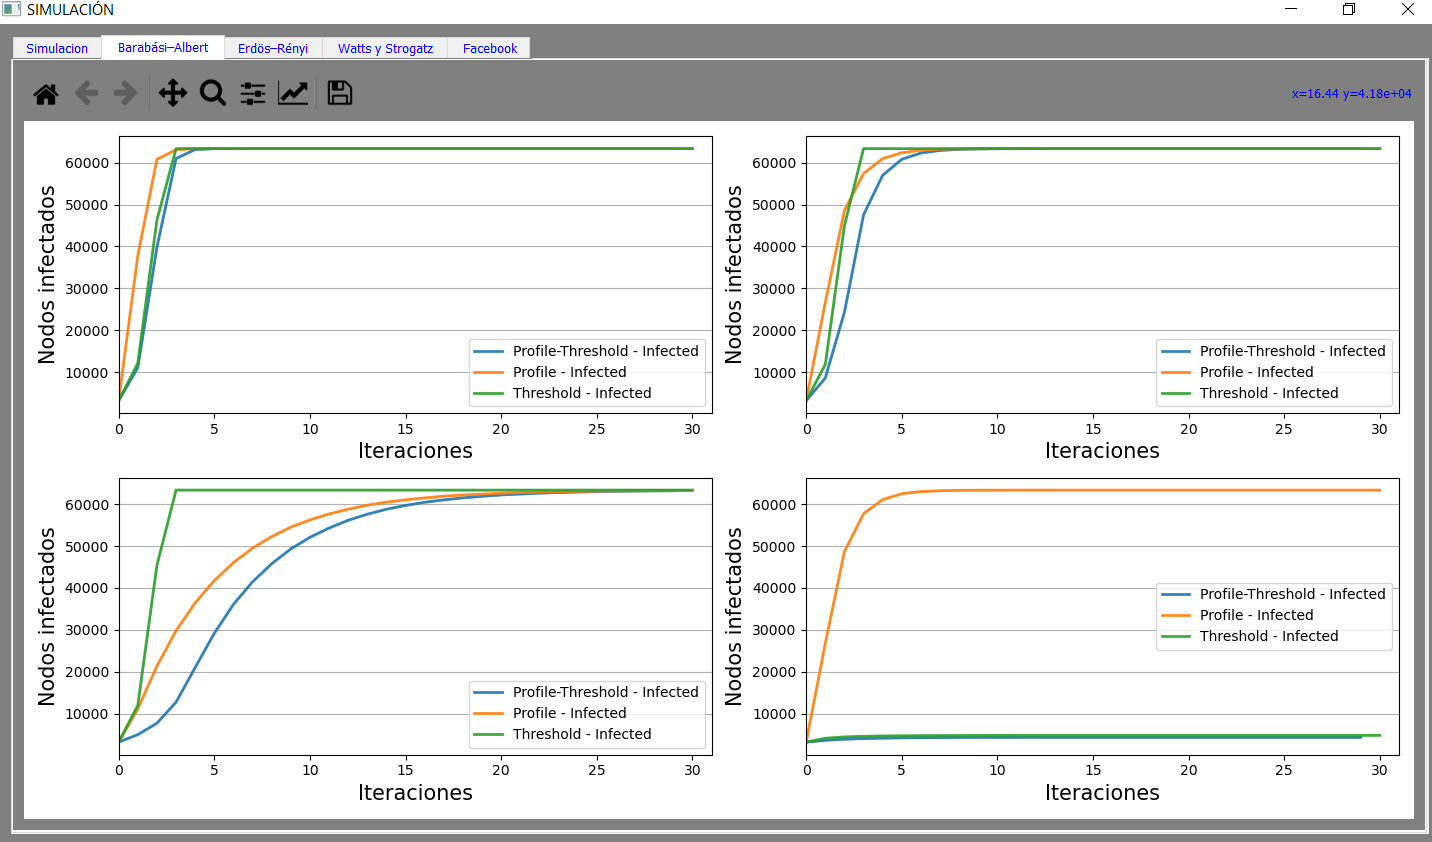
\includegraphics[width=\textwidth]{../Images/GUI_1.PNG}
		\caption{}
		\label{fig:gui1}
	\end{subfigure}
	\begin{subfigure}[b]{1\textwidth}
		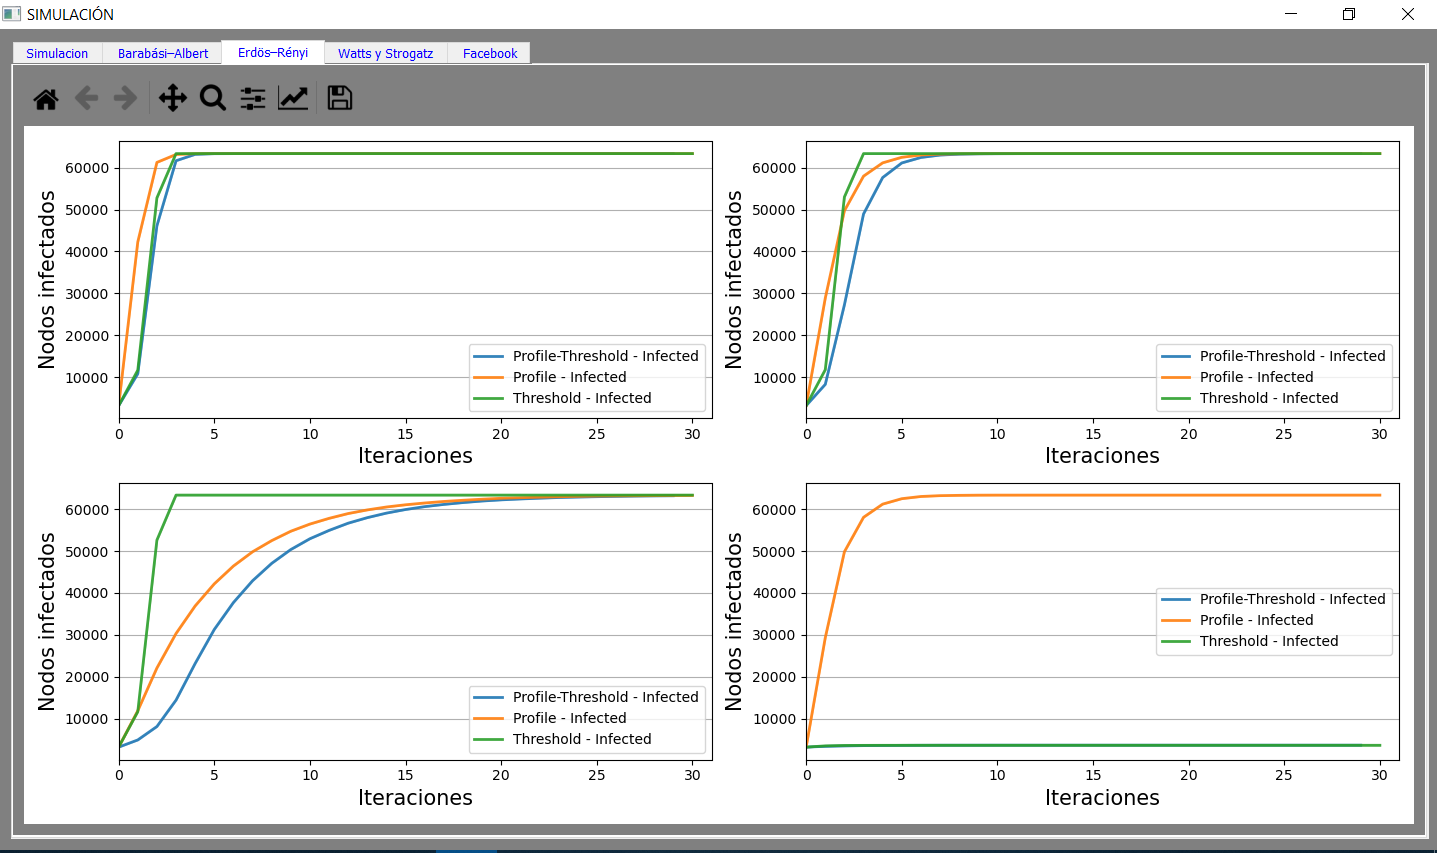
\includegraphics[width=\textwidth]{../Images/GUI_2.PNG}
		\caption{}
		\label{fig:gui2}
	\end{subfigure}
	\label{fig:graficas}
	\caption{Interfaz grafica donde se muestran las graficas para los resultados de los grafos de Barabási-Albert y Erdós Renyi.}
\end{figure}

\begin{figure}[!tbp]
	\begin{subfigure}[b]{1\textwidth}
		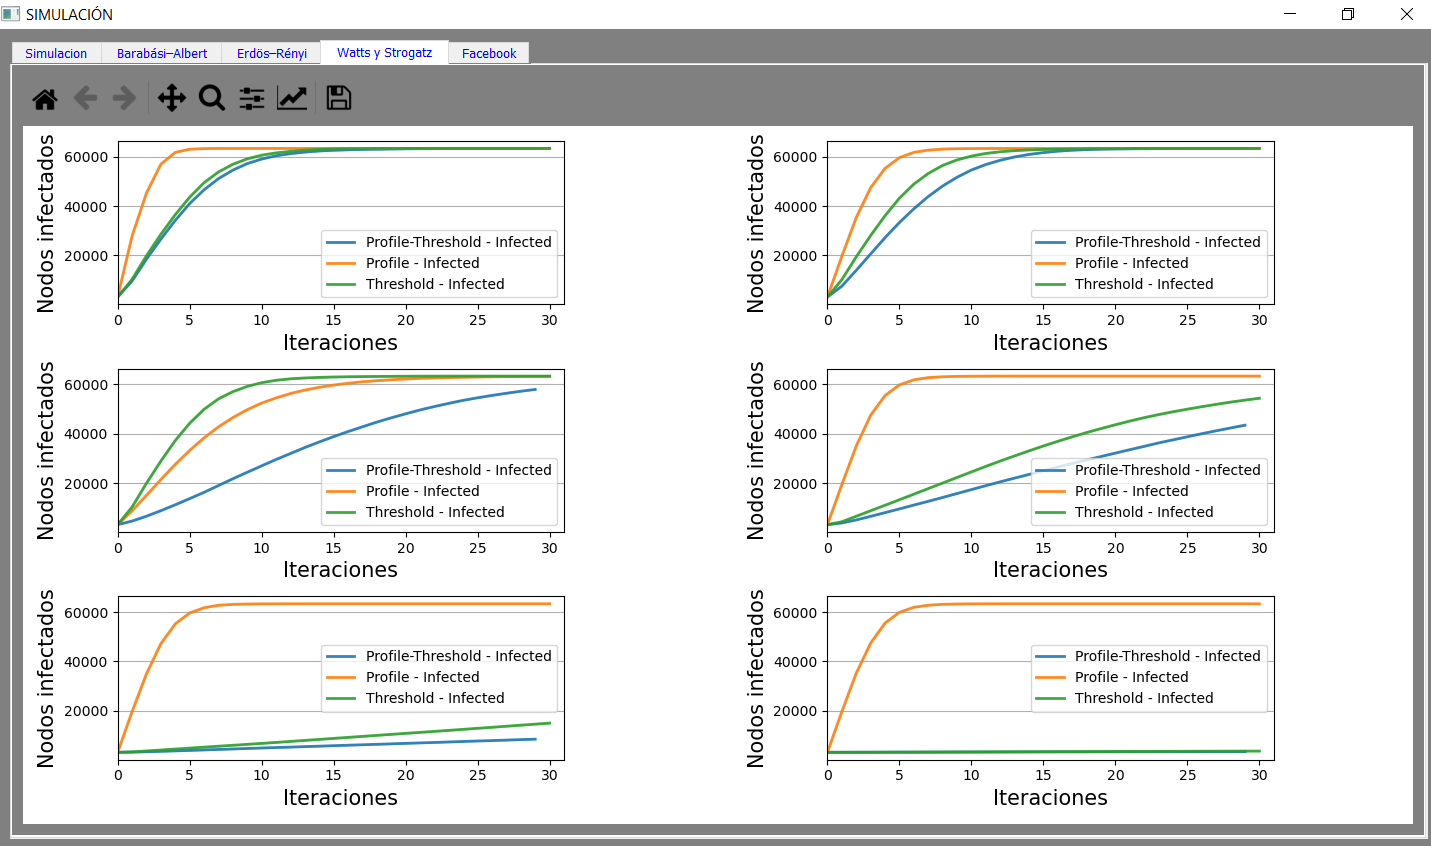
\includegraphics[width=\textwidth]{../Images/GUI_3.PNG}
		\caption{}
		\label{fig:gui3}
	\end{subfigure}
	\hfill
	\begin{subfigure}[b]{1\textwidth}
	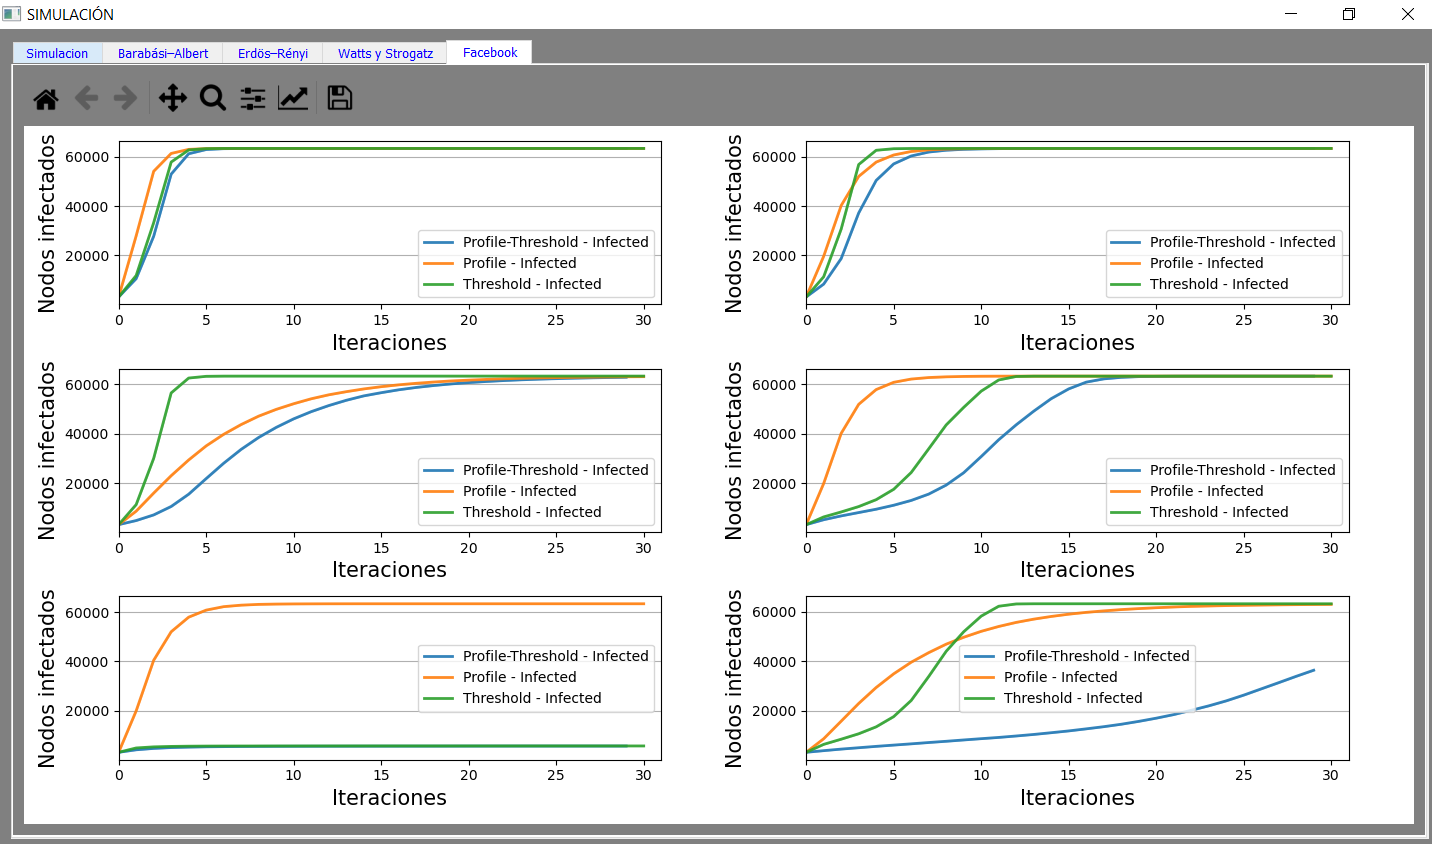
\includegraphics[width=\textwidth]{../Images/GUI_4.PNG}
	\caption{}
	\label{fig:gui4}
	\end{subfigure}
	\label{fig:graficas}
	\caption{Interfaz grafica donde se muestran las graficas para los resultados del grafo de Wats-Strogatz y Facebook.}
\end{figure}
\newpage
\section{Validación}
\subsection{Protocolo de Analisis}
Para realizar la validación y experimentación del modelo, así como para comparar los escenarios de difusión descritos anteriormente, diseñamos los siguientes protocolo analítico:
\begin{itemize}
\item Para cada conjunto de datos, seleccionamos al azar 100 conjuntos de nodos, cada uno cubriendo el $5\%$ de $V$: Dichos conjuntos identifican, para cada escenario y modelo, $100$ semillas iniciales de infección diferentes configuración - $I_0$
\item Para cada conjunto de datos, escenario y $I_0$ se ejecutan los modelos de difusión activa, pasiva y mixta con 30 iteraciones cada uno.
\item Comparamos los modelos analizando las tendencias de infección obtenidas así como el porcentaje de nodos infectados al final de cada simulación.
\end{itemize}
Para comprender el impacto que tienen los diferentes valores de los parámetros del modelo en el proceso de difusión, simulamos los tres escenarios con varias configuraciones del threshold del nodo, $\iota$, y node profile $\iota$. Además, también se varia el valor de probabilidad de inmunización $p$, y tasa de adopción espontánea $a$. Como resultado, instanciamos todos las combinaciones de parámetros para los modelos seleccionados, variando sus valores en los siguientes rangos:

\begin{itemize}
\item Threshold, $t$ : [0.1, 0.2, 0.3, 0.4, 0.5, 0.6, 0.7, 0.8]
\item Node Profile, $\iota$ : [0.05, 0.1, 0.2, 0.3, 0.4, 0.5, 0.6, 0.7, 0.8]
\item Porcentaje de nodos bloqueados $p$: [0, 0.1, 0.2, 0.3]
\item Probabilidad de adopción espontanea, $a$: [0, 0.001, 0.005, 0.01]
\end{itemize}
\newpage
\subsection{Resultados}

No se implementa interfaz para mostrar los mapas de calor generados, ya que el consumo de recursos que utiliza para realizar todas las simulaciones es demasiado elevado y además el poder generar los mapas de calor requiere de alto tiempo de ejecución, un promedio de 1.5 hr por mapa de calor. A pesar de eso, se muestran las imagenes generadas sobre estos y por otra parte, las graficas si se muestran en interfaz 


Para caracterizar mejor los resultados obtenidos analizamos por separado los modelos que contemplan nodos bloqueados de los que no lo hacen. Tratamos de forma similar los resultados obtenidos en presencia / ausencia de adopciones espontáneas.

\textbf{1. Sin inmunización, sin adopciones espontáneas.}\\
En este escenario cae la implementación estándar de los tres métodos; Analizamos redes por separado para caracterizar mejor las diferencias entre los métodos.

\textbf{Grafo de Barabási-Albert}
\\
En la $Figura$ $3$ se puede apreciar los resultados obtenidos de las tendencias de difusión al aplicar los tres modelos en la red generada mediante el algoritmo de Barabási-Albert. 
\begin{itemize}
	\item En la $Figura$ $\ref{fig:f1}$ se puede observar que al fijar los umbrales $\tau = 0.1$ y los valores de los perfiles del nodo $\gamma = 0.1$ se obtiene que las tendencias de los tres modelos son similares.
	\item En la $Figura$ $\ref{fig:f2}$ se puede observar que al fijar los umbrales $\tau = 0.1$ y los valores de los perfiles del nodo $\gamma = 0.4$ se observa que los tres modelos a la cuarta iteración tienen a la mayor parte de la red como infectados, aunque el modelo $Threshold$ tiende a hacelo más rapido.
	\item En la $Figura$ $\ref{fig:f3}$ se puede observar que al fijar los umbrales $\tau = 0.1$ y los valores de los perfiles del nodo $\gamma = 0.8$ se observa que el modelo $Threshold$ es el más rapido en realizar la infección de la red en pocas iteraciones y los otros dos se mantienten similares.
	\item En la $Figura$ $\ref{fig:f4}$ se puede observar que al fijar los umbrales $\tau = 0.2$ y los valores de los perfiles del nodo $\gamma = 0.4$ se observa notablemente que el modelo $Threshold$ se mantiene como el más rapido para infectar, debido a que la presión del exterior es significativa o tiende a ser superior a tus ideales, es decir, eres influenciados por la presión de otros.
\end{itemize}


\begin{figure}[!tbp]
	\begin{subfigure}[b]{0.5\textwidth}
		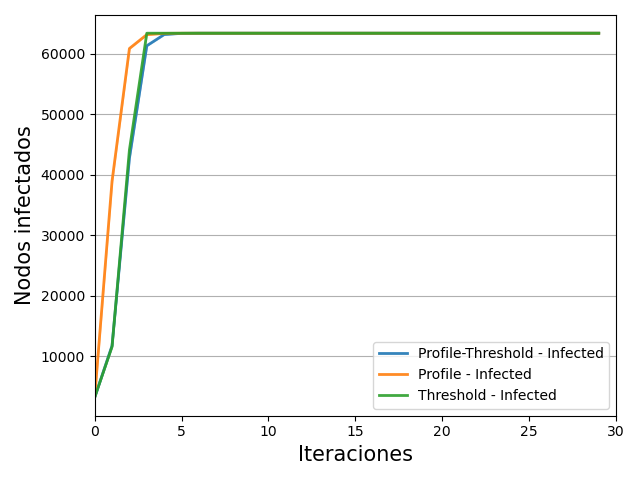
\includegraphics[width=\textwidth]{../Images/Fig 1 a).png}
		\caption{}
		\label{fig:f1}
	\end{subfigure}
	\hfill
	\begin{subfigure}[b]{0.5\textwidth}
		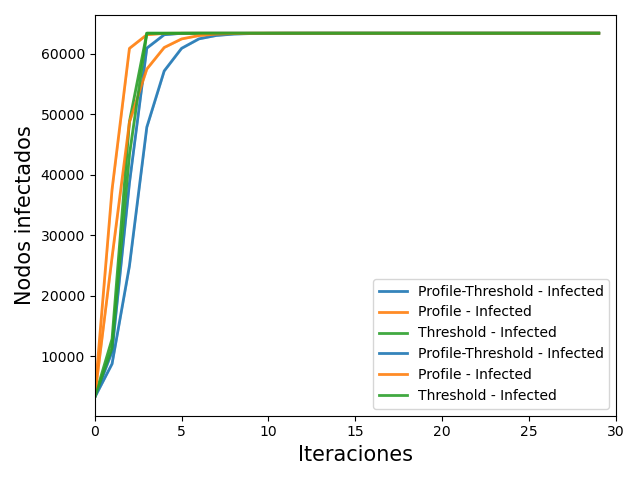
\includegraphics[width=\textwidth]{../Images/Fig 1 b).png}
		\caption{}
		\label{fig:f2}
	\end{subfigure}
		\begin{subfigure}[b]{0.5\textwidth}
		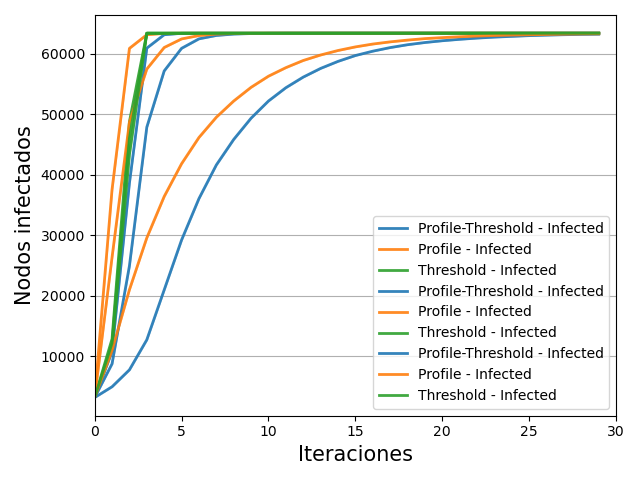
\includegraphics[width=\textwidth]{../Images/Fig 1 c).png}
		\caption{}
		\label{fig:f3}
	\end{subfigure}
	\hfill
	\begin{subfigure}[b]{0.5\textwidth}
		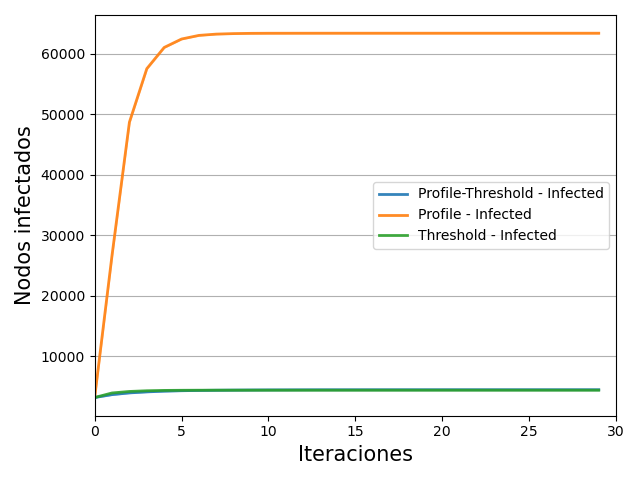
\includegraphics[width=\textwidth]{../Images/Fig 1 d).png}
		\caption{}
		\label{fig:f4}
	\end{subfigure}
	\label{fig:FIG1}
	\caption{Tendencias de difusión del grafo Barabási-Albert. Tendencias de difusión para los modelos Threshold, ProfileThreshold y Profile con a = 0 y p = 0 y con diferentes valores de $\gamma$ y $\tau$. \textbf{a} $\gamma$ = 0.1, $\tau$ = 0.1 \textbf{b} $\gamma$ = 0.4, $\tau$ = 0.1 \textbf{c} $\gamma$ = 0.8, $\tau$ = 0.1 \textbf{d} $\gamma$ = 0.4, $\tau$ = 0.2}
\end{figure}
\newpage
\textbf{Grafo de Erdós-Renyi}
En la $Figura$ $4$ se puede apreciar los resultados obtenidos de las tendencias de difusión al aplicar los tres modelos en la red generada mediante el algoritmo de Erdós-Renyi. 
\begin{itemize}
	\item Lo que se puede observar de todas las subfiguras es que son muy similiares a las obtenidas en la $Figura$ $3$, por lo que no queda más por detallar sobre esto.
\end{itemize}

\begin{figure}[!tbp]
	\begin{subfigure}[b]{0.5\textwidth}
		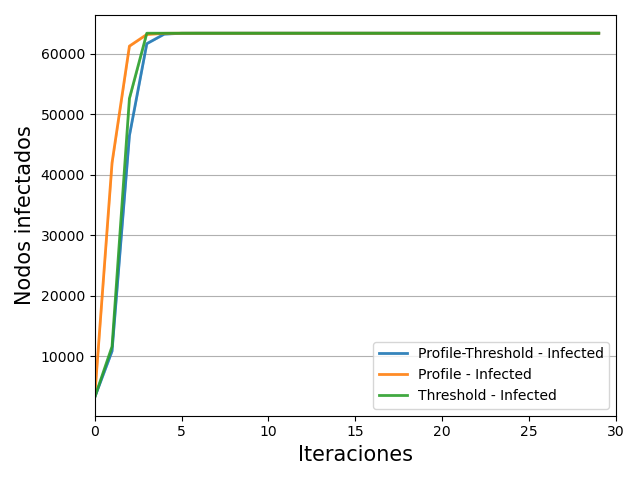
\includegraphics[width=\textwidth]{../Images/Fig 2 a).png}
		\caption{}
		\label{fig:f21}
	\end{subfigure}
	\hfill
	\begin{subfigure}[b]{0.5\textwidth}
		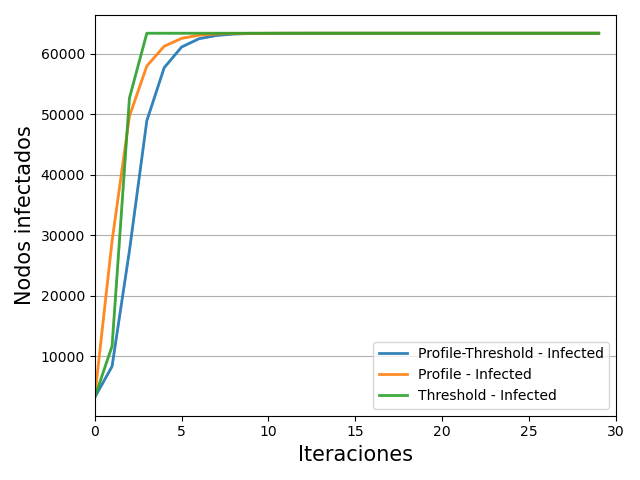
\includegraphics[width=\textwidth]{../Images/Fig 2 b).png}
		\caption{}
		\label{fig:f22}
	\end{subfigure}
	\begin{subfigure}[b]{0.5\textwidth}
		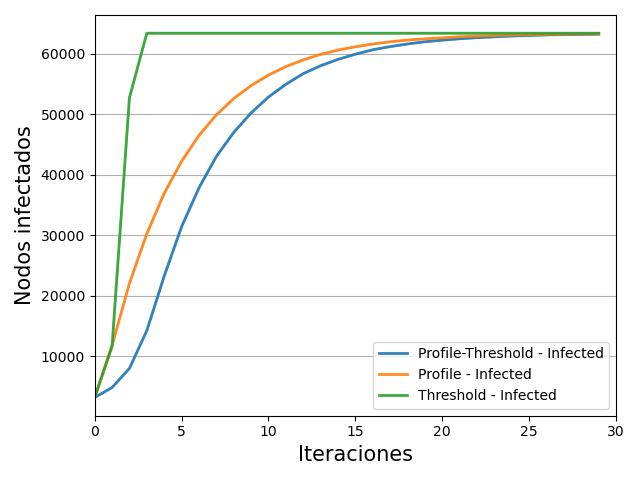
\includegraphics[width=\textwidth]{../Images/Fig 2 c).png}
		\caption{}
		\label{fig:f23}
	\end{subfigure}
	\hfill
	\begin{subfigure}[b]{0.5\textwidth}
		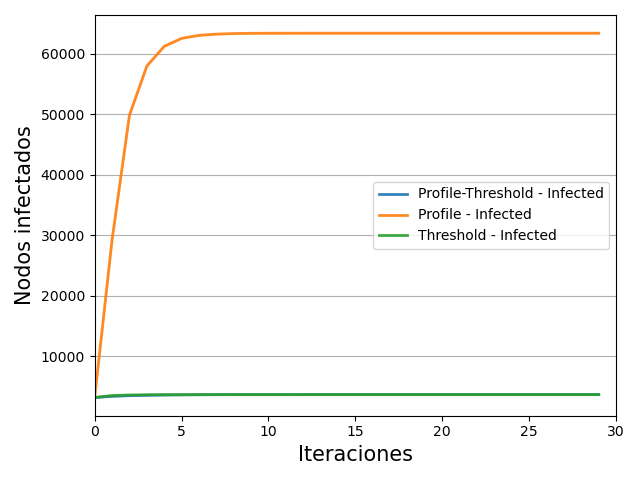
\includegraphics[width=\textwidth]{../Images/Fig 2 d).png}
		\caption{}
		\label{fig:f24}
	\end{subfigure}
	\label{fig:FIG2}
	\caption{Tendencias de difusión del grafo Erdós-Renyi. Tendencias de difusión para los modelos Threshold, ProfileThreshold y Profile con a = 0 y p = 0 y con diferentes valores de $\gamma$ y $\tau$. \textbf{a} $\gamma$ = 0.1, $\tau$ = 0.1 \textbf{b} $\gamma$ = 0.4, $\tau$ = 0.1 \textbf{c} $\gamma$ = 0.8, $\tau$ = 0.1 \textbf{d} $\gamma$ = 0.4, $\tau$ = 0.2}
\end{figure}
\newpage
\textbf{Grafo de Wats-Strogatz}
En la $Figura$ $5$ se puede apreciar los resultados obtenidos de las tendencias de difusión al aplicar los tres modelos en la red generada mediante el algoritmo de Wats-Strogatz. 

\begin{itemize}
	\item En la $Figura$ $\ref{fig:f31}$ se puede observar que al fijar los umbrales $\tau = 0.1$ y los valores de los perfiles del nodo $\gamma = 0.1$ se obtiene que el modelo de $Profile$ realiza las infecciones de forma más rapida y los modelos restantes lo hacen de forma similiar y más lento.
	\item En la $Figura$ $\ref{fig:f32}$ se puede observar que al fijar los umbrales $\tau = 0.1$ y los valores de los perfiles del nodo $\gamma = 0.4$ se obtiene que el modelo de $Profile$ se mantiene como el más rapido para realizar las infecciones y que despues lo hace el modelo $Threshold$ de forma más lenta y finalmente el modelo $Profile-Threshold$ el más lento de los tres.
	\item En la $Figura$ $\ref{fig:f33}$ se puede observar que al fijar los umbrales $\tau = 0.1$ y los valores de los perfiles del nodo $\gamma = 0.8$ se obtiene que el modelo de $Profile$ es superado por el modelo $Threshold$ a pesar de que se aumenta el valor para los perfiles del nodo, donde se estimaría que fuese mayor el $Profile$. El modelo restante se mantiene como el más lento de infección.
	\item En la $Figura$ $\ref{fig:f34}$ se puede observar que al fijar los umbrales $\tau = 0.2$ y los valores de los perfiles del nodo $\gamma = 0.4$ se obtiene que el modelo de $Profile$ vuelve a superar por mucho al modelo $Threshold$ y este a su vez al $Profile-Threshold$, se aprecia que el modelo $Profile$ es más rapido y los otros tan lentos que no alcanzan a contagiar toda la red.
	\item En la $Figura$ $\ref{fig:f35}$ se puede observar que al fijar los umbrales $\tau = 0.3$ y los valores de los perfiles del nodo $\gamma = 0.4$ se obtiene que el modelo de $Profile$ contagia a toda la red de forma muy rapida y los modelos restantes no alcanzan ni a poder contagiar el 20\% de esta.
	\item En la $Figura$ $\ref{fig:f35}$ se puede observar que al fijar los umbrales $\tau = 0.3$ y los valores de los perfiles del nodo $\gamma = 0.4$ se obtiene que el modelo de $Profile$ contagia a toda la red de forma muy rapida y los modelos restantes no alcanzan a contagiar ni al 7\% de la población total, considerando además que el 5\% ya lo estaba, entonces se vuelven más reales al detallar resultados.
\end{itemize}


\begin{figure}[!tbp]
	\begin{subfigure}[b]{0.5\textwidth}
		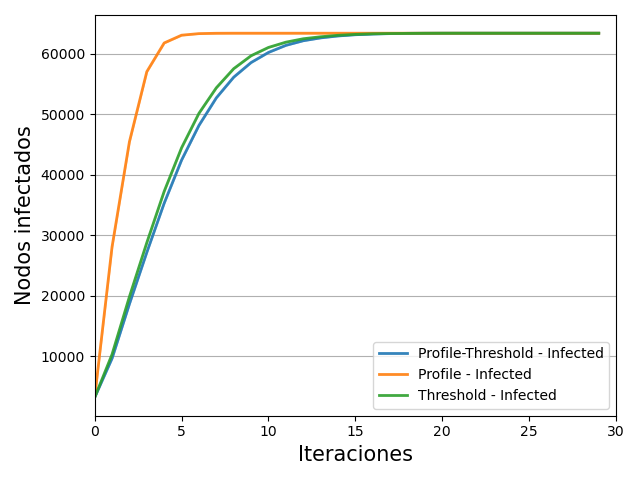
\includegraphics[width=\textwidth]{../Images/Fig 3 a).png}
		\caption{}
		\label{fig:f31}
	\end{subfigure}
	\hfill
	\begin{subfigure}[b]{0.5\textwidth}
		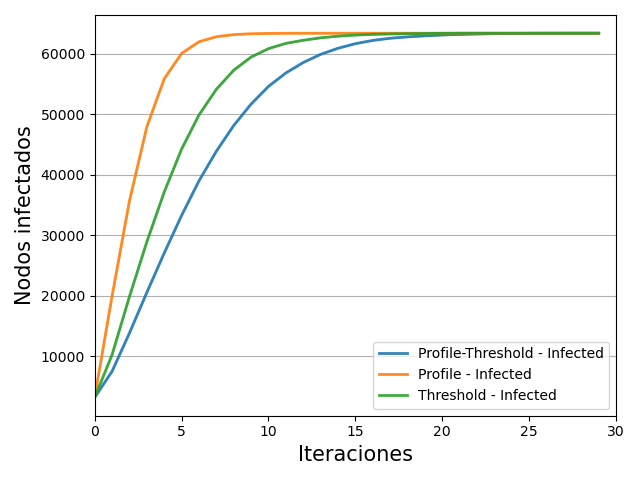
\includegraphics[width=\textwidth]{../Images/Fig 3 b).png}
		\caption{}
		\label{fig:f32}
	\end{subfigure}
	\begin{subfigure}[b]{0.5\textwidth}
		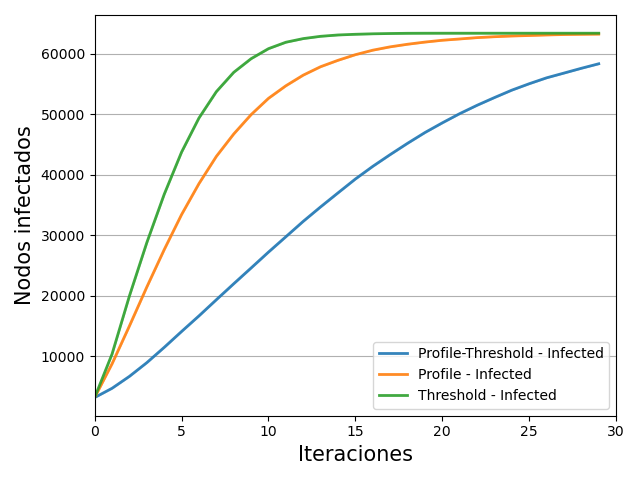
\includegraphics[width=\textwidth]{../Images/Fig 3 c).png}
		\caption{}
		\label{fig:f33}
	\end{subfigure}
	\hfill
	\begin{subfigure}[b]{0.5\textwidth}
		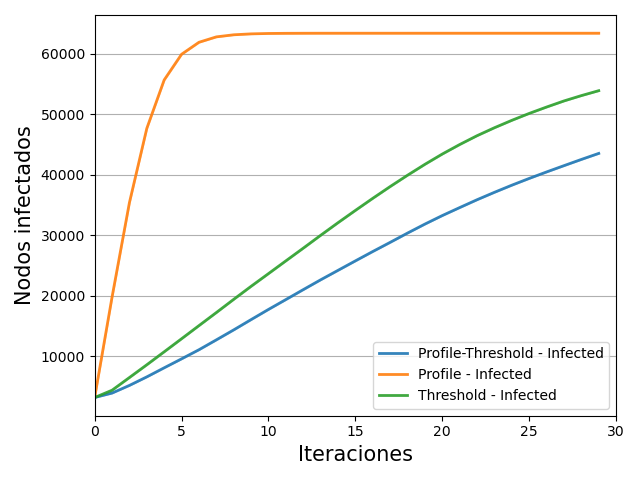
\includegraphics[width=\textwidth]{../Images/Fig 3 d).png}
		\caption{}
		\label{fig:f34}
	\end{subfigure}
	\hfil
	\begin{subfigure}[b]{0.5\textwidth}
		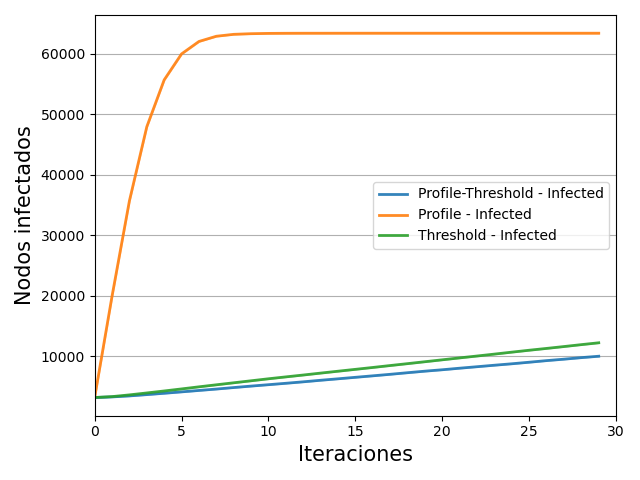
\includegraphics[width=\textwidth]{../Images/Fig 3 e).png}
		\caption{}
		\label{fig:f35}
	\end{subfigure}
	\hfill
	\begin{subfigure}[b]{0.5\textwidth}
		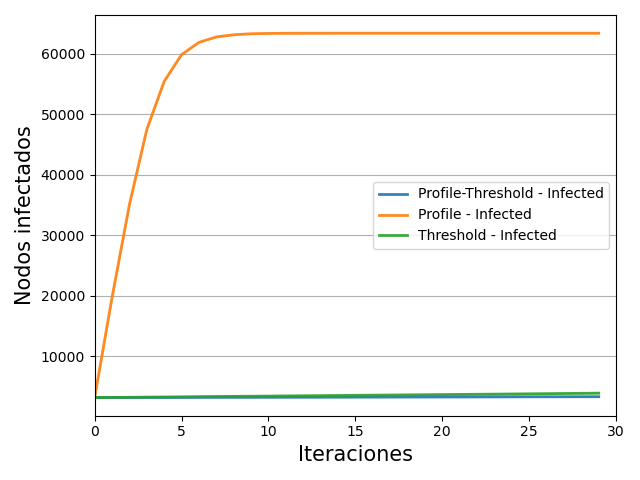
\includegraphics[width=\textwidth]{../Images/Fig 3 f).png}
		\caption{}
		\label{fig:f36}
	\end{subfigure}
	\label{fig:FIG3}
	\caption{Tendencias de difusión del grafo Wats-Strogatz. Tendencias de difusión para los modelos Threshold, ProfileThreshold y Profile con a = 0 y p = 0 y con diferentes valores de $\gamma$ y $\tau$.
		\textbf{a} $\gamma$ = 0.1, $\tau$ = 0.1 \textbf{b} $\gamma$ = 0.4, $\tau$ = 0.1 \textbf{c} $\gamma$ = 0.8, $\tau$ = 0.1 \textbf{d} $\gamma$ = 0.4, $\tau$ = 0.2 \textbf{e} $\gamma$ = 0.4, $\tau$ = 0.3 \textbf{f} $\gamma$ = 0.4, $\tau$ = 0.4}
\end{figure}

\textbf{Grafo de Facebook}


En la $Figura$ $6$ se puede apreciar los resultados obtenidos de las tendencias de difusión al aplicar los tres modelos en la red real generada mediante los datos de Facebook. 

\begin{itemize}
	\item Los resultados que se obtienen son similares a los de los grafos sinteticos, inclusive se puede apreciar como una mezcla de ellos. Por ejemplo, las $Figuras $ \ref{fig:f41}, \ref{fig:f42}, \ref{fig:f43} es muy similar a las $Figuras $ \ref{fig:f1}, \ref{fig:f2}, \ref{fig:f3}. 
	\item Por el resto, también se puede apreciar que realmente el modelo más lento para realizar el contagio de toda la red es el $Profile-Threshold$.
\end{itemize}


\begin{figure}{c}
	\label{fig:plot4}
	\begin{subfigure}[b]{0.5\textwidth}
		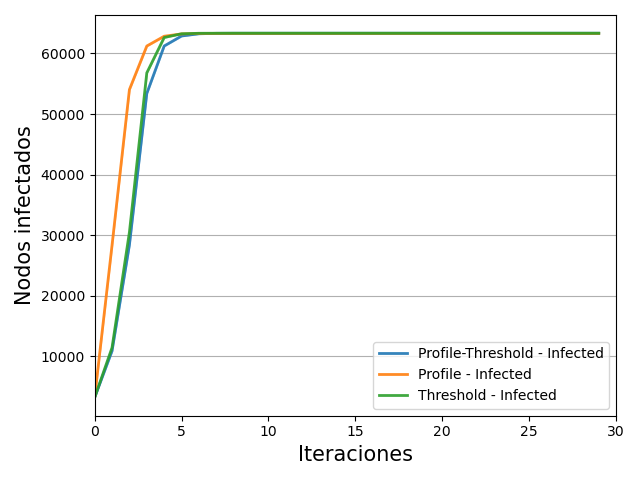
\includegraphics[width=\textwidth]{../Images/Fig 4 a).png}
		\caption{}
		\label{fig:f41}
	\end{subfigure}
	\hfill
	\begin{subfigure}[b]{0.5\textwidth}
		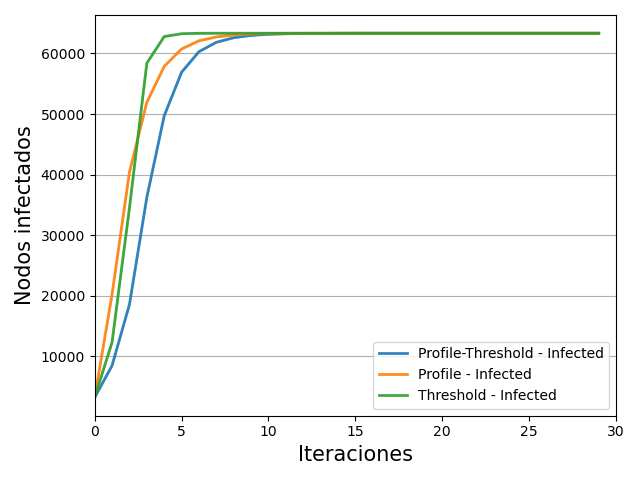
\includegraphics[width=\textwidth]{../Images/Fig 4 b).png}
		\caption{}
		\label{fig:f42}
	\end{subfigure}
	\begin{subfigure}[b]{0.5\textwidth}
		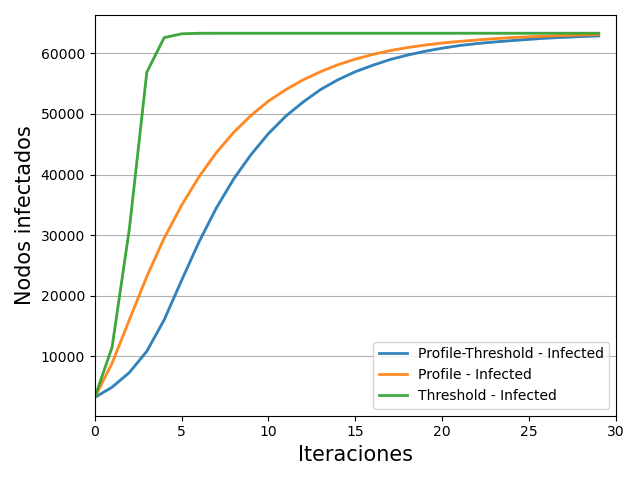
\includegraphics[width=\textwidth]{../Images/Fig 4 c).png}
		\caption{}
		\label{fig:f43}
	\end{subfigure}
	\hfill
	\begin{subfigure}[b]{0.5\textwidth}
		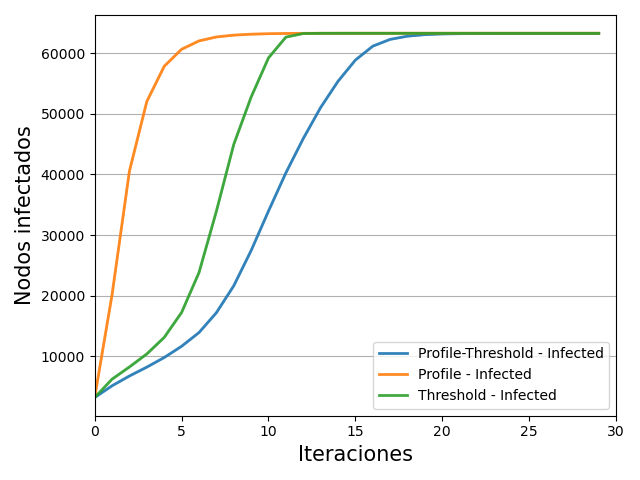
\includegraphics[width=\textwidth]{../Images/Fig 4 d).png}
		\caption{}
		\label{fig:f44}
	\end{subfigure}
	\hfil
	\begin{subfigure}[b]{0.5\textwidth}
		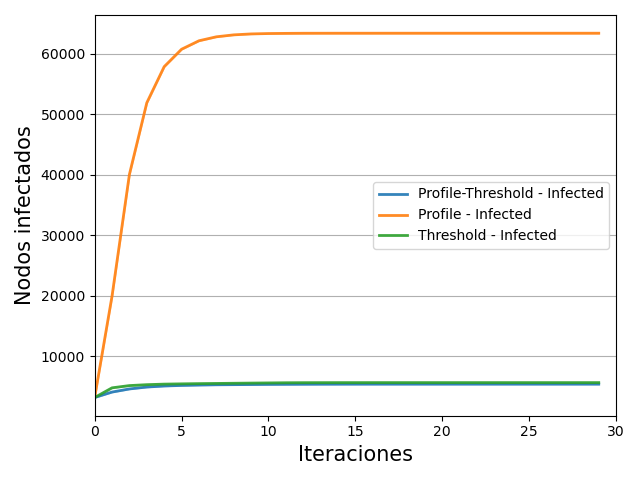
\includegraphics[width=\textwidth]{../Images/Fig 4 e).png}
		\caption{}
		\label{fig:f45}
	\end{subfigure}
	\hfill
	\begin{subfigure}[b]{0.5\textwidth}
		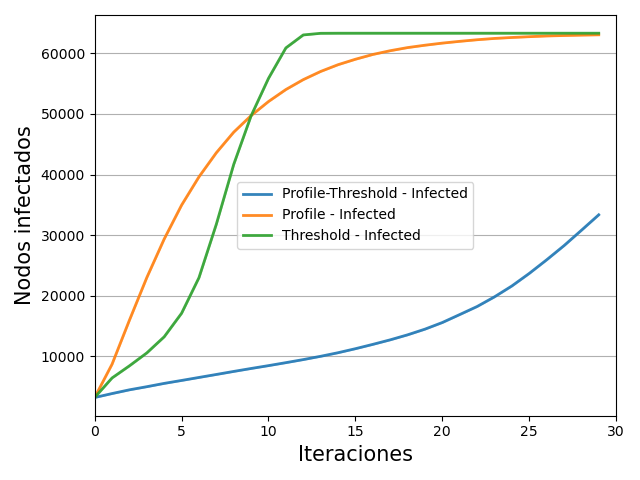
\includegraphics[width=\textwidth]{../Images/Fig 4 f).png}
		\caption{}
		\label{fig:f46}
	\end{subfigure}
	\caption{Tendencias de difusión del grafo de Facebook. Tendencias de difusión para los modelos Threshold, ProfileThreshold y Profile con a = 0 y p = 0 y con diferentes valores de $\gamma$ y $\tau$.\textbf{a} $\gamma$ = 0.1, $\tau$ = 0.1 \textbf{b} $\gamma$ = 0.4, $\tau$ = 0.1 \textbf{c} $\gamma$ = 0.8, $\tau$ = 0.1 \textbf{d} $\gamma$ = 0.4, $\tau$ = 0.2 \textbf{e} $\gamma$ = 0.4, $\tau$ = 0.3 \textbf{f} $\gamma$ = 0.8, $\tau$ = 0.2}
\end{figure}

De las graficas presentadas y especificamente de las últimas dos, correspondiente al grafo de $Facebook$ y $Wats-Strogatz$, se muestra que la difusión con el compartamiento $activo$ se realizan de forma más rapida y el $pasivo$ pasa a la inversa, la tendencia de difusión progresa de forma más lenta. Y en general lo resultados son los esperados, el modelo $Profile$ y $Threshold$ realizan de forma más rapida las tendencias difusión, mientras el $Profile-Threshold$ en las dos primeras redes sinteticas se comportó igual que los demás, es decir, los escenarios $mixto$ y $pasivo$ se comportaron de forma similar; en la red de $Wats-Strogatz$ y $Facebook$ se observó con mejor claridad que el modelo realizaba las tendencias de difusión mucho más lento y por debajo al modelo $Threshold$.

El modelo $Profile-Threshold$ es más lento debido a que primero el nodo tiene que superar el umbral de exposición para poder estar en contacto con la información y posteriormente decidir por su propia cuenta si lo acepta o lo declina, entonces requiere de tener una cantidad de vecinos infectados relativamente alta y posteriormente tener que decidir adquirir la información porque lo desea o es de su agrado. 

\newpage
\textbf{2. Sin inmunización, con adopciones espontáneas.}

Este escenario se simuló aplicando los tres modelos presentados anteriormente en el grafo creado con los datos reales de $Facebook$ y son representados los resultados en mapas de calor, así como se muestra en las $Figuras$: $7$, $8$, $9$. 

\begin{figure}[h]
	\begin{subfigure}[b]{0.5\textwidth}
		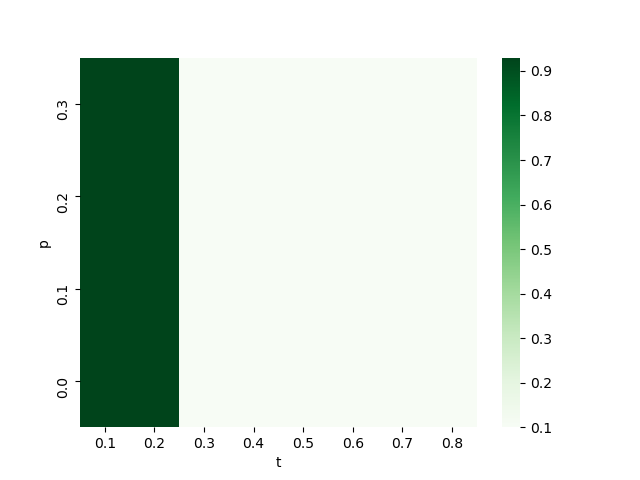
\includegraphics[width=\textwidth]{../Images/hm01.png}
		\caption{a = 0}
		\label{fig:hm01}
	\end{subfigure}
	\hfill
	\begin{subfigure}[b]{0.5\textwidth}
		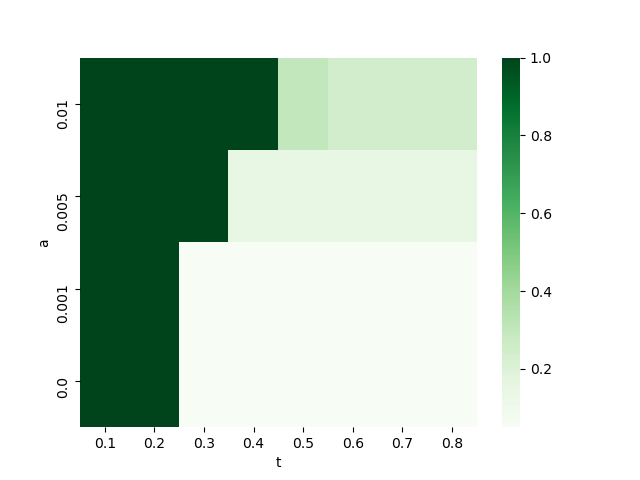
\includegraphics[width=\textwidth]{../Images/hm02.png}
		\caption{p = 0}
		\label{fig:hm02}
	\end{subfigure}
	\hfill
	\begin{subfigure}[b]{0.5\textwidth}
		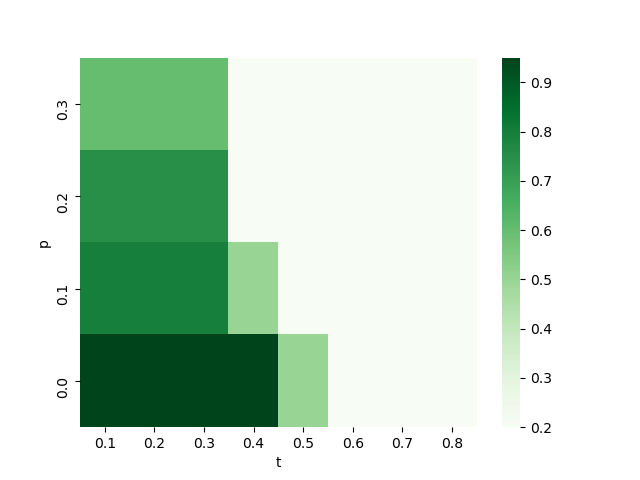
\includegraphics[width=\textwidth]{../Images/hm03.png}
		\caption{a = 0.01}
		\label{fig:hm03}
	\end{subfigure}
	\begin{subfigure}[b]{0.5\textwidth}
		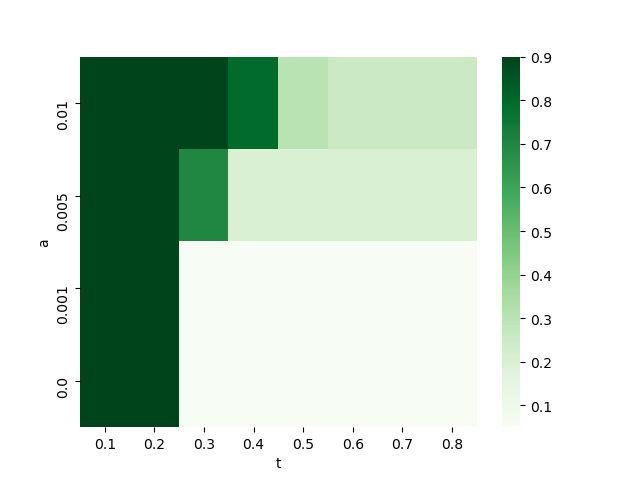
\includegraphics[width=\textwidth]{../Images/hm04.png}
		\caption{p = 0.1}
		\label{fig:hm04}
	\end{subfigure}
	\label{fig:hm}
	\caption{Mapas de calor obtenidos al aplicar el modelo $Threshold$, el eje x corresponde a la variable $\tau$ que corresponde a los umbrables del nodo, y en \textbf{a} y \textbf{c} se varia el valor de la probabilidad de inmunización $p$, mientras que en \textbf{b} y \textbf{d} se varia el valor de adopción $a$.}
\end{figure}
Cada celda de un mapa de calor representa el porcentaje de nodos infectados al final de una simulación. Si la celda tiene un color azul fuerte esto representa un porcentaje alto y si es color más claro de azul representa un valor bajo.
\newpage

\textbf{3. Con inmunización, sin adopciones espontáneas.}

En este escenario se agrega el concepto de nodos bloqueados y se ve como los patrones de la difusión cambian. Para las simulaciones, se considera la elección de nodos bloqueados de forma random. Para el modelo de $Profile$ $Figura $ \ref{fig:hm05}, se puede observar que después del mismo período el porcentaje de nodos infectados se reduce a la mitad en comparación con la simulación con $p = 0$, ya que en este escenario se descarta la adopciones espontáneas $a$.

\begin{figure}[h]
	\begin{subfigure}[b]{0.5\textwidth}
		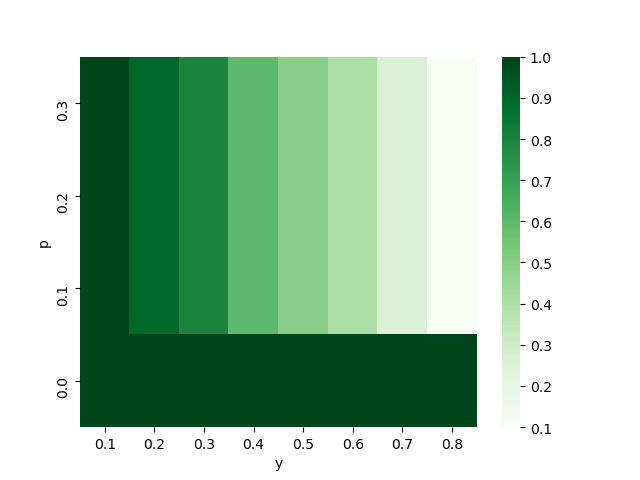
\includegraphics[width=\textwidth]{../Images/hm05.png}
		\caption{a = 0}
		\label{fig:hm05}
	\end{subfigure}
	\hfill
	\begin{subfigure}[b]{0.5\textwidth}
		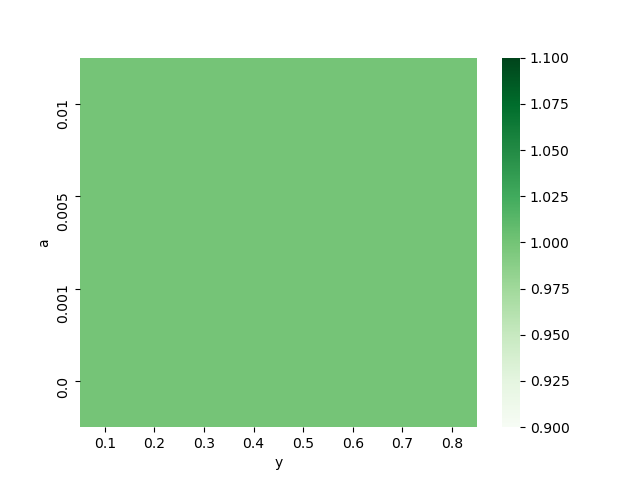
\includegraphics[width=\textwidth]{../Images/hm06.png}
		\caption{p = 0}
		\label{fig:hm06}
	\end{subfigure}
	\hfill
	\begin{subfigure}[b]{0.5\textwidth}
		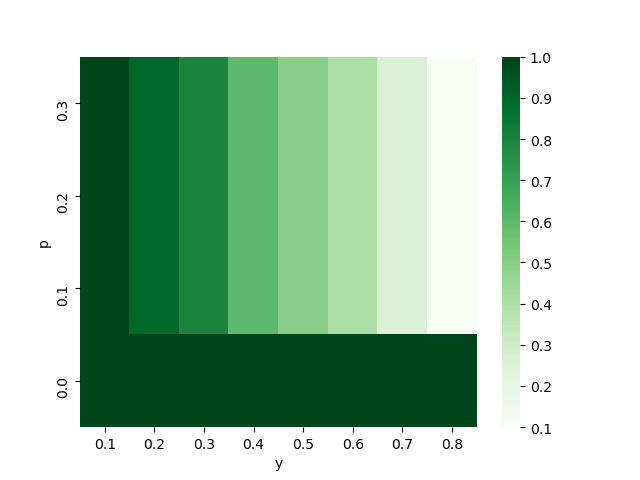
\includegraphics[width=\textwidth]{../Images/hm07.png}
		\caption{a = 0.01}
		\label{fig:hm07}
	\end{subfigure}
	\begin{subfigure}[b]{0.5\textwidth}
		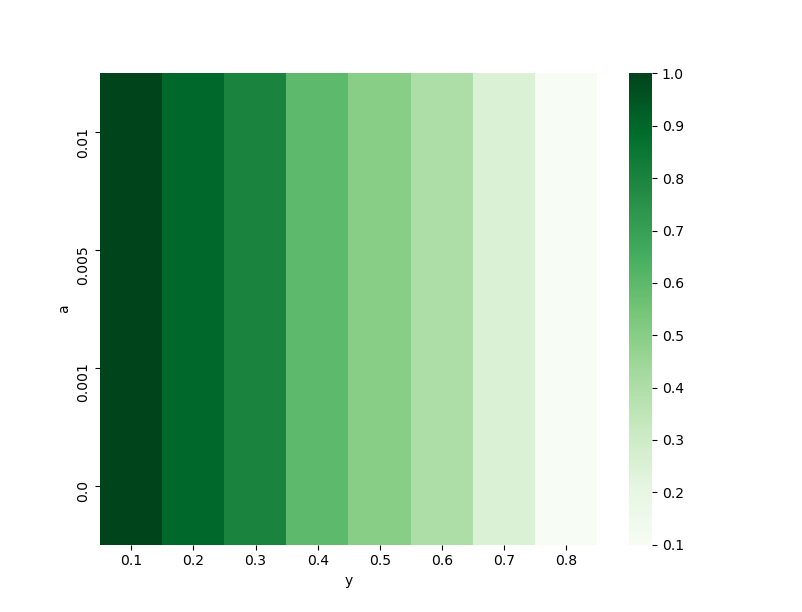
\includegraphics[width=\textwidth]{../Images/hm08.png}
		\caption{p = 0.1}
		\label{fig:hm08}
	\end{subfigure}
	\label{fig:hm2}
	\caption{Mapas de calor obtenidos al aplicar el modelo $Profile$, el eje x corresponde a la variable $\gamma$ que corresponde a los perfiles del nodo, y en \textbf{a} y \textbf{c} se varia el valor de la probabilidad de inmunización $p$, mientras que en \textbf{b} y \textbf{d} se varia el valor de adopción $a$.}
\end{figure}

\newpage
\textbf{4. Con inmunización, con adopciones espontáneas.}

En este escenario hay variaciones a la variable $p$ correspondiente a la inmutizacion de los nodos (nodos bloqueados) y la variable $a$ que indica las adopciones espontáneas. Se puede observar de las $Figuras: $ \ref{fig:hm03}, \ref{fig:hm04}, \ref{fig:hm07}, \ref{fig:hm08}, \ref{fig:hm11}, \ref{fig:hm12} que cada vez que aumenta el valor de $a$ el porcentaje de nodos infectados también crece, y al inversa sucede cuando el valor de $p$ aumenta, el porcentaje de nodos infectados decrece.
\begin{figure}[h]
	\begin{subfigure}[b]{0.5\textwidth}
		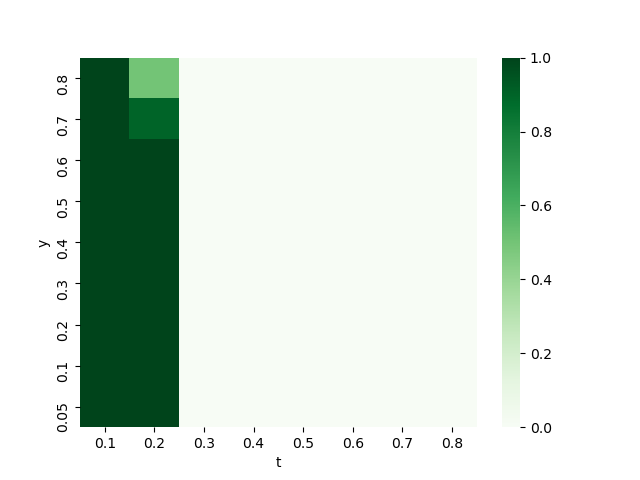
\includegraphics[width=\textwidth]{../Images/hm09.png}
		\caption{p = 0, a = 0}
		\label{fig:hm09}
	\end{subfigure}
	\hfill
	\begin{subfigure}[b]{0.5\textwidth}
		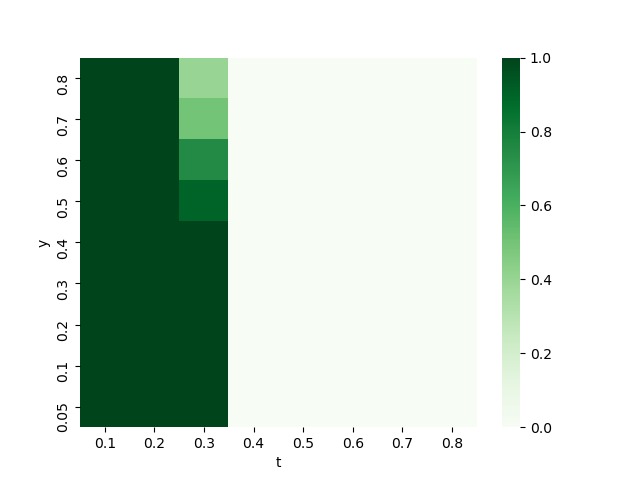
\includegraphics[width=\textwidth]{../Images/hm10.png}
		\caption{p = 0, a = 0.005}
		\label{fig:hm10}
	\end{subfigure}
	\hfill
	\begin{subfigure}[b]{0.5\textwidth}
		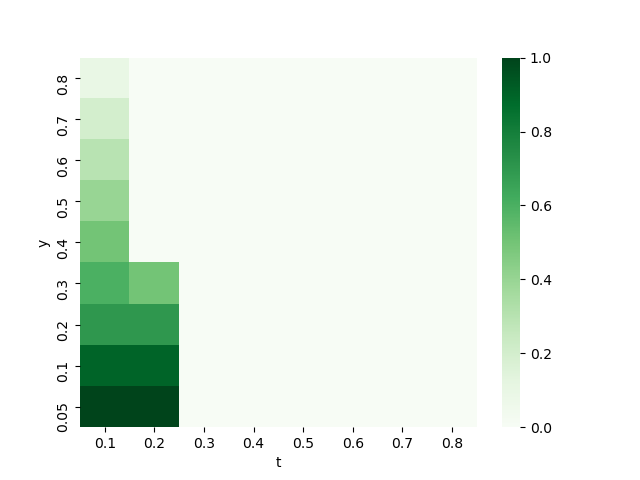
\includegraphics[width=\textwidth]{../Images/hm11.png}
		\caption{p = 0-2, a = 0}
		\label{fig:hm11}
	\end{subfigure}
	\begin{subfigure}[b]{0.5\textwidth}
		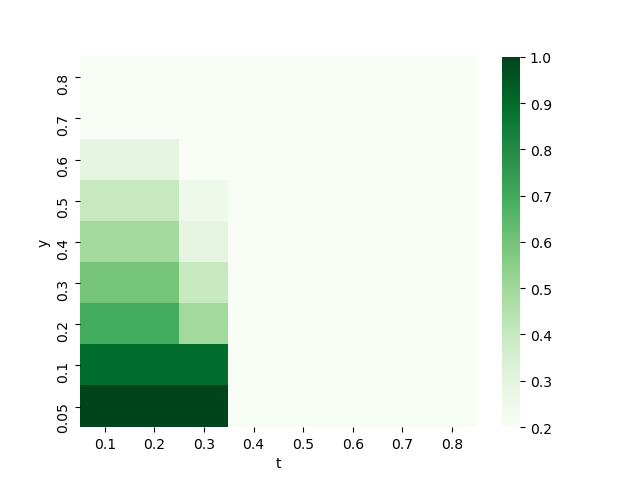
\includegraphics[width=\textwidth]{../Images/hm12.png}
		\caption{p = 0.2, a = 0.005}
		\label{fig:hm12}
	\end{subfigure}
	\label{fig:hm3}
	\caption{Mapas de calor obtenidos al aplicar el modelo $Profile-Threshold$, el eje x corresponde a la variable $\tau$ que corresponde a los umbrales del nodo y el en eje y se matiene a $\gamma$ que son los perfiles del nodo.}
\end{figure}
\newpage
\section{Conclusiones}
En el trabajo se abordó el problema de actividades en la difusión de información, en el que se simularon diferentes escenarios en el que se pusieron a prueba tres modelos de simulación propuestos que entran en un marco de modelado común. En comparación de los modelos compartimentales (SI, SIR, SIS), el modelo $Threshold$ dado un estado de infección inicial (seed) produce una evolución determinista de la difusión, haciéndole falta un detonador estocástico, la difusión que produce este modelo se puede observar como un modelo $pasivo$ ya que los nodos involucrados no juegan un papel importante al momento de determinar si son o no infectados, es decir, no están con un rol activo. Se puede denotar rápidamente que el modelo $Threshold$ es eficiente para simular redes en las que la presión social es un factor y las preferencias individuales no lo son, es decir, una red donde las personas son influenciadas por el medio que lo rodea.



Posterior a este modelo, se proponen dos modelos con simulación estocástica que incluyen una participación activa del nodo involucrado, estos modelos son: $Profile$ y $Profile-Threshold$. De las pruebas realizadas con escenarios de $pasivo$ y $activo$ se pudo visualizar como influenciaba cada parámetro a que la tendencia de difusión fuera más rápida o más lenta, entonces al combinar los dos escenarios, se pudo notar que al realizar la simulación los resultados eran más reales, debido a que se consideraba la presión del exterior y los intereses individuales.



Además en los escenarios propuestos, se agregó la presencia de adoptantes espontáneos (indivudos infectados de por factores exógenos) y también los nodos bloqueados, que estos representaban a individuos que se negaban a adoptar/cambiar de opinión sobre un contenido o ser influenciado, estos parámetros ayudaron a acelerar/amortiguar el proceso de la difusión según los valores que tuvieran. De los dos modelos propuestos, se notó que el más eficiente para realizar la simulación y el que mejores resultados reales presentaba, era el modelo $Profile-Threshold$, que es un modelo con condiciones más fuertes de cumplir y es por ello que se vuelve más complicado de realizar las tendencias de difusión, además que se vuelve más apegado a la realidad; es mejor debido a que considera factores externos al individuo y también los intereses del mismo.
	
	Gracias a este trabajo, se puede apreciar la importancia de la simulación, ya que en base a modelos de este tipo, se puede simular y obtener resultados para poder visualizar el comportamiento de un evento del mundo real. En este caso fue de una red compleja de individuos en la que se difundía información pero de igual forma puede ser aplicado para simular la dispersión de un virus biológico, virus informatico, información, etc. y son de ayuda para poder proyectar resultados a futuro y realizar analisis y en base a estos tomar decisiones. También se notó la importancia que tiene el poder diseñar un modelo eficaz, ya que en nuestro caso el modelo $Threshold$ que habían propuesto hace tiempo, era un modelo que realizaba simulación tipo $determinista$ y entonces los resultados eran poco reales debido a que consideraba menos parametros y su enfoque no era el adecuado, pero al reformular este modelo y proponer nuevos, los resultados que se simulaban era mejores y se veían más reales, debido a que ahora la simulación era de tipo estocástica, entonces es ahí la importancia del poder formular un buen modelo, ya que nuestros resultados pueden no ser los esperados o los correctos y apegados a la realidad.
	 
\newpage

\printbibliography

\end{document}